\chapter{Automated Discovery of Failure Domain+ and Daikon to Analyse Failure Boundaries}
\label{chap:ADFD+}



\section{Introduction}\label{sec:intro}
Testing is the most widely used and essential method of software testing. Ample efforts have been made to improve its effectiveness and efficiency. Testing is effective if it finds maximum number of faults in minimum number of test cases. Testing efficiency is the process to execute maximum number of test cases in minimum possible time. It is concluded that automation is the key to achieve both effectiveness and efficiency of software testing. Automation of a single part like data generation, execution, oracle or the whole system is highly beneficial in most of the cases. Some of the common automated testing tools include YETI~\cite{Oriol2011yeti}, Randoop~\cite{pacheco2007randoop}, Eclat~\cite{pacheco2005eclat}, QuickCheck~\cite{claessen2011quickcheck} and Jaretege~\cite{oriat2005jartege}. 

Daikon~\cite{ernst2007daikon} is one of the several tools, which uses machine learning technique to automatically generate likely invariants of the program written in C, C++, Java and Pearl. Daikon takes as input the program and few test cases written manually or generated by an automated tool. It executes the test cases on the program under test and observes the values that the program computes. At the end of the test session it reports the properties that were true over the observed executions. Daikon can process the generated invariants to mitigate non interesting and redundant invariants. Daikon can also inserts the generated invariants in to the source code as assertions. Daikon's output can be useful in understanding program, generating invariants, predicting incompatibilities in component integration, automating theorem proving, repairing inconsistent data structures and checking the validity of data streams.

While the idea behind Daikon is attractive, it is interesting to see how much the auto generated invariants represent the fault domain residing in the program. To assess this, we set up performed several experiments and analysed the results derived from the error-seeded programs tested with Daikon and ADFD+. ADFD+ is a framework named Automated Discovery of Failure Domain+. It is based on our previous strategy Automated Discovery of Failure Domain (ADFD), which tries to find a fault, search the surrounding for more faults and graphically plot the fault domain if any~\cite{ahmad2013adfd}.  

The main contribution of the article are:
\begin{itemize}
\item \textbf{ADFD+:} It brings some changes to the previously proposed ADFD strategy. The new strategy improves the search algorithm of ADFD and make the report more intuitive.
\item \textbf{Implementation of ADFD+:} The new ADFD+ strategy is implemented and integrated in the YETI tool.
\item \textbf{Evaluation:} It evaluates the report generated by Daikon and ADFD+ about the boundaries known fault domains in the error-seeded programs. It is found that where Daikon was able to find the fault, it was not able to identify its domain boundary as accurately as ADFD+.
\item \textbf{Future work:} It gives ideas of further application of ADFD+, such as finding and plotting faults in multi-dimensional programs using multi-dimensional graphs. 
% A case study suggesting that boundaries are properly recognized by Daikon and ADFD+ or Daikon lake .... etc.
\end{itemize}
%The rest of this paper is organised as follows: \\ Section~\ref{sec:adfd} describes the ADFD+ strategy. Section~\ref{sec:imp} presents implementation of the ADFD+ strategy. Section~\ref{sec:eval} explains the experimental setup. Section~\ref{sec:res} shows results of the experiments. Section~\ref{sec:discussion} discusses the results. Section~\ref{sec:rw} presents related work and Section~\ref{sec:conc}, concludes the study.


%In the later part we plot the domain on the basis of invariants generated by Daikon and compare both the domains.

%%%%%%%%%%%%%%%%%    Background   %%%%%%%%%%%%%%%%%%%

\section{Failure Patterns}
A number of empirical evidence confirms that fault revealing test cases tend to cluster in contiguous regions across the input domain~\cite{white1980domain, finelli1991nasa, schneckenburger2007towards}. According to Chan et al.~\cite{chan1996proportional} the clusters are arranged in the form of point, block and strip failure pattern. In the point pattern the failure revealing inputs are stand alone which are spread through out the input domain. In block pattern the failure revealing inputs are clustered in a one or more contiguous area. Finally, in strip pattern the failure revealing inputs are clustered in one long elongated area.  Figure~\ref{fig:failurePatterns} shows the failure patterns in two-dimensional input domain. 

\begin{figure}[ht]                                    
\centering
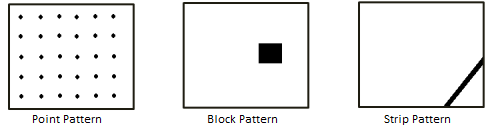
\includegraphics[width= 8cm,height=2.5cm]{ART_Patterns.png}
\caption{Failure patterns across input domain~\cite{chan1996proportional}}
\label{fig:failurePatterns}
\end{figure}

%In Section~\ref{sec:adfd+} we describe the ADFD+ framework that can find the failure, its domain and plot the domain up to the specified range in a graphical form. Experiments confirms the successful working of ADFD+.


 

%%%%%%%%%%%%%%%%%    ADFD+   %%%%%%%%%%%%%%%%%%%

\section{Automated Discovery of Failure Domain+}\label{sec:adfd+}
ADFD+ is an improved and extended form of our previously developed Automated Discovery of Failure Domain~\cite{ahmad2013adfd}. The ADFD+ is an automated framework that finds the failures, their domains in a specified range and present them on a graphical chart. Following  are the main differneces between ADFD and ADFD+.

\begin{itemize}
\item ADFD+ generate a single Java file dynamically at run time to plot the failure domains instead of one Java file per failure as in ADFD. This saves a lot of execution time and makes the process much quicker.

\item ADFD+ uses (x, y) vector series to represent failure pattern as opposed to the (x, y) line series in ADFD. The vector series allows more flexibility and clarity to represent a failure and its domain domain.   

\item ADFD+ takes a single value as range which specify a round region around the failure whereas takes two values for lower and upper bound representing x and y axis respectively.

\item In ADFD+, the algorithm of dynamically generated Java file, which is created after an error is discovered, is made more simplified and efficient.

\item In ADFD+, the failure domain is focused in the graph which gives a clear view of pass and fail points. The points are also labelled for simplification as shown in the Figure~\ref{fig:Workflow}. 

%The difference in representation of fault by ADFD and ADFD+ can be seen in figure .... Figure x is generated by ADFD with lower bound as ... and upper bound as ... While Figure Y is generated by ADFD+ with range ... for the same program given in appendix a. 
\end{itemize}


%%%%%%%%%%%%%%%%%%%%

\subsection{Workflow of ADFD+}
ADFD+ is an automatic process and all the user has to do is to specify the program to test and click the $Draw Fault Domain$ button. The default value for range is set to 5 which means that ADFD+ will search 25 values around the failure. On clicking the button YETI is executed with ADFD+ strategy to search for a failure. On finding a failure the ADFD+ strategy create a java file which contain calls to the program on the failing value and related values up to the specified range. The Java file is compiled and executed. The result is analysed to check for pass and failed values. Pass values are stored in pass file and fail values are stored in fail file. At the end of the values range, the values are plotted on the graph with pass values as green and fail values as red as shown in the Figure~\ref{fig:Workflow}.


%Instead of front end give workflow. It will make more sense. Change the code of the program

\begin{figure}[ht]
\centering
\includegraphics[width= 8.5cm,height=6.5cm]{adfdPlusWorkflow.png}
\caption{Workflow of ADFD+}
\label{fig:Workflow}
\end{figure}


%%%%%%%%%%%%%%%%%%%%
%ADFD+ is an extension of ADFD's algorithm with more accuracy to find and clarity to plot the failure domain on a graphical chart. Deriving failure domains using ADFD+ is a one click process and all the tester needs to input is the class to test and the range-value for which to search around the found failure. 
%%%%%%%%%%%%%%%%%%%%

\subsection{Implementation of ADFD+}
The ADFD+ strategy is implemented in a tool called York 
Extensible Testing Infrastructure (YETI). YETI is available 
in open-source at \url{http://code.google.com/p/yeti-test/}. In this section a brief overview of YETI is given with the focus on the parts relevant to the implementation of ADFD+ strategy. For verification of ADFD+ strategy in YETI, a program is used 
as an example to illustrate the working of ADFD+ strategy. Please refer to \cite{Oriol2011yeti, oriol2012random, oriol2010testing, oriol2010yeti} for more details on YETI. 

YETI is a testing tool developed in Java that test programs using random strategies in an automated fashion. YETI meta-model is language-agnostic which enables it to test 
programs written in functional, procedural and object-oriented languages. 

YETI consists of three main parts including core infrastructure for extendibility through specialization, strategies section for adjustment of multiple strategies and 
languages section for supporting multiple languages. Both the languages and strategies sections have a pluggable architecture to easily incorporate new strategies and 
languages making YETI a favorable choice to implement ADFD+ strategy. YETI is also capable of generating test cases to reproduce the faults found during the test session. 
The strategies section in YETI contains all the strategies including random, random+ and DSSR to be selected for testing according to the specific needs. The default test 
strategy for testing is random. On top of the hierarchy in strategies, is an abstract class YetiStrategy, which is extended by YetiRandomPlusStrategy and is further, extended to get 
ADFD+ strategy.


\subsection{ADFD+ by an example}
In this section we describe the working of ADFD+ with a motivating example. Suppose we have the following class name $Error$ under test. According to the code, the value of variable $x$ between 5 to 8 and the value of variable $y$ between 2 to 4 triggers a failure.   

\begin{lstlisting}

public class Error {

  public static void Error (int x, int y){

    int z;

    if (((x>=5)&&(x<=8))&&((y>=2)&&(y<=4)))
		 {
			 z = 50/0;
		 }
   } 
}
\end{lstlisting}

On execution, the ADFD+ strategy tests the class with the help of YETI and finds the first failure at x = 6 and y = 3. Once a failure is discovered ADFD+ uses the surrounding values around it to find a failure domain. The range of surrounding values is limited to the value set by the user in the $Domain Range$ variable. When the value of $Domain Range$ is 5, ADFD+ evaluates total of 83 values of $x$ and $y$ around the found failure. All evaluated (x, y) values are plotted on a two dimensional graph with red dot indicating a failing value and green dot indicating the passing value. Figure~\ref{fig:adfdPlusExample} clearly show that the failure domain forms a block pattern and the boundaries of the failure are $(5, 2), (5, 3),(5, 4), (6, 2), (6, 4), (7, 2), (7, 4), (8, 2), (8, 3), (8, 4)$.

\begin{figure*}[ht]
\centering
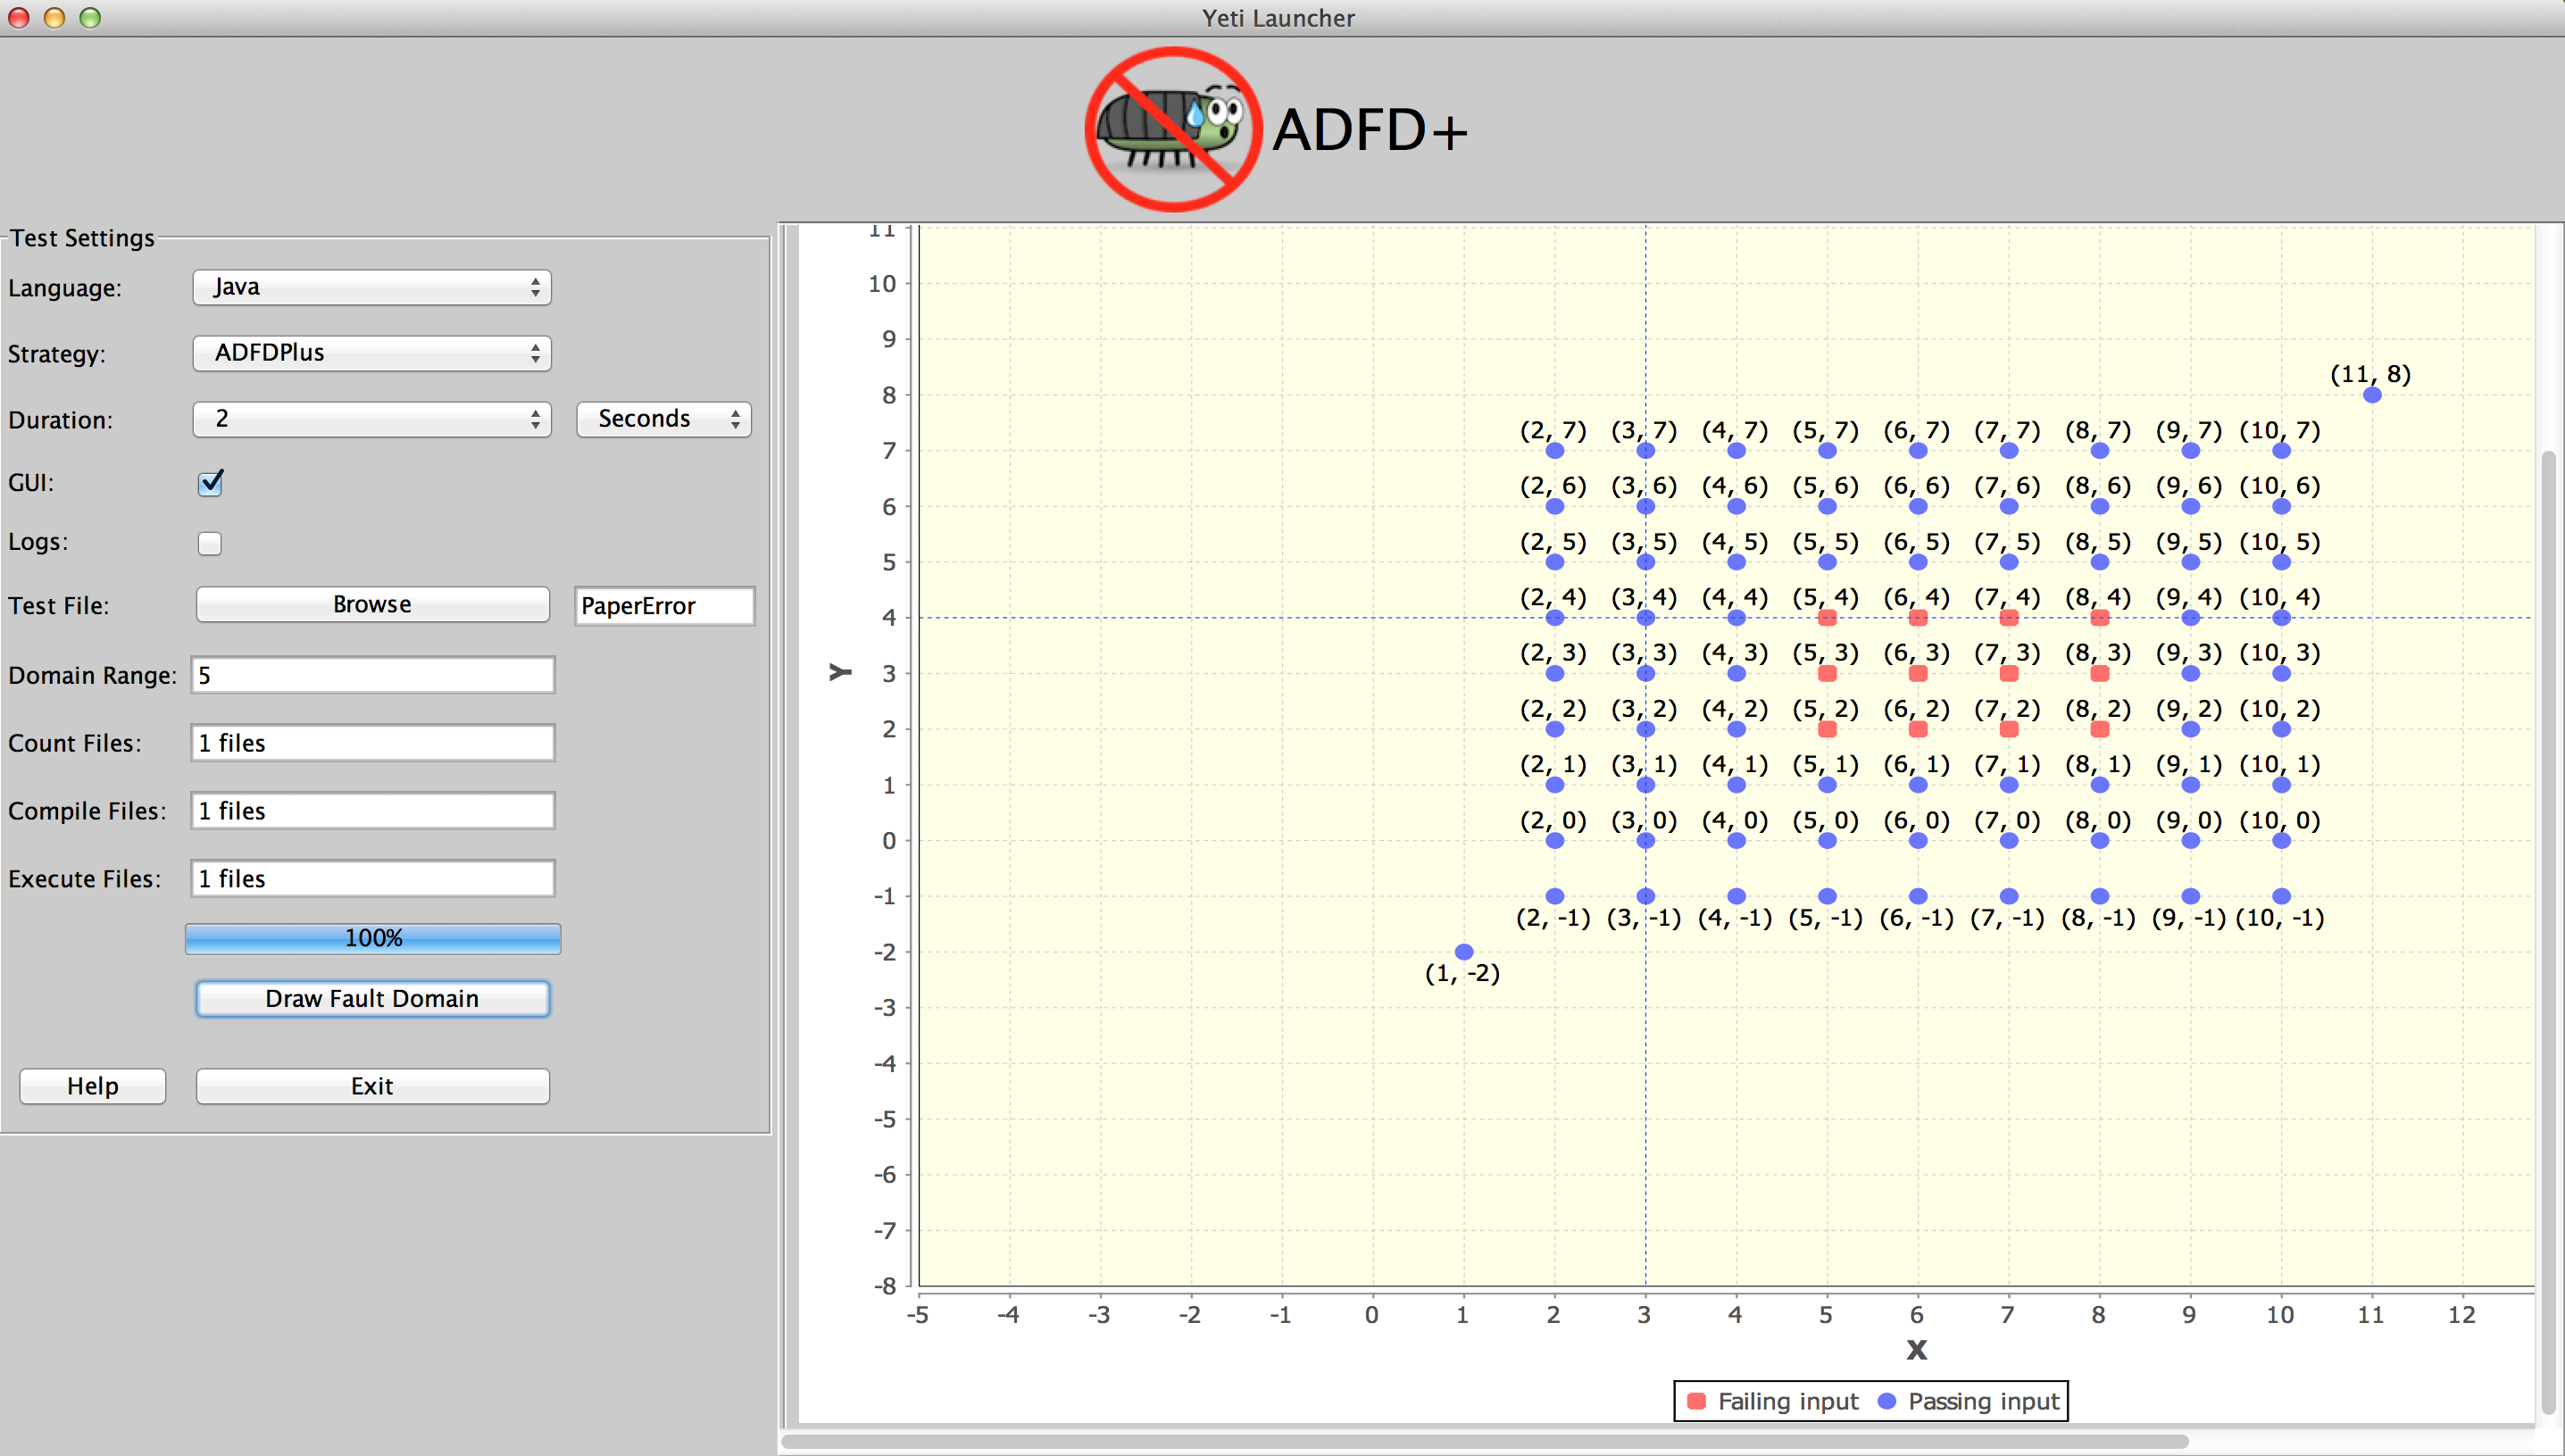
\includegraphics[width=17.5cm,height=11cm]{exampleError.png}
\caption{The output of ADFD+ for the above code.}
\label{fig:adfdPlusExample}
\end{figure*}









%%%%%%%%%%%%%%%%%    EVALUATION   %%%%%%%%%%%%%%%%%%%%


\section{Evaluation}\label{sec:eval}
Because of using error-seeded one and two dimensional numerical programs, we were aware of the failure domain present in each program. The correct identification and presentation of the failure domain by ADFD+ prove the correct working of ADFD+. We then evaluated the same program by Daikon and plot its results. The unit test cases required by Daikon for generating invariants were generated using Randoop~\cite{}. YETI being capable of generating the test cases is not used for this step to keep the second completely independent from first. 

\subsection{Research questions}
For evaluating Daikon, the following research questions have been addressed in this study:
\begin{enumerate}
\item If Daikon is capable of generating invariants to identify the failure?
\item If Daikon is capable of generating invariants that identify the failure domain?
\item If Daikon is capable of correctly identifying the boundaries of the failure domain?
\end{enumerate}

\subsection{Experiments}
To evaluate the Daikon performance for failure domain, we performed testing of several error seeded one and two dimensional numerical programs written in Java. All the selected programs were seeded with at least one failure domain of point, block or strip nature. Every program is tested twenty times by both ADFD+ and Daikon. The program code is given in Appendix~\ref{} while the test details is presented in Table~\ref{table:Results}.

Every class is evaluated through $10^5$ calls in each test session of ADFD+.
%\footnote{The total number of tests is equal to $60\times 30\times 3 \times 10^5 = 540\times10^6~tests$.} 
Because of the absence of the contracts and assertions in the code under test, similar approach as used in previous studies ~\cite{Oriol2012} is followed using undeclared exceptions to compute failures.


All tests are performed with a 64-bit Mac OS X Lion Version 10.7.4 running on 2 x 2.66 GHz 6-Core Intel Xeon processor with 6 GB (1333 MHz DDR3) of RAM. YETI runs on top of the Java\texttrademark  SE Runtime Environment [version 1.6.0\_35]. The machine took approximately 100 hours to process the experiments.

\section{results}

for point, block and strip of one dimensional program. Use the same programs of ADFD, same figures but analyse it again on Daikon. because ADFD and ADFD+ behave in the same way for one dimension.

For point block and strip of two dimensional programs. Use adfd+ system.






\section{Discussion}
\section{Threats to validity}




\section{Conclusion}

\section{Future Work}
to extend ADFD+ to multidimensional non numerical programs.
